\chapter{Mélanger et dissoudre}\label{ch:g2:mixing-and-dissolving}

Un morceau de sucre tombe dans une tasse de thé chaud. Une cuillère
tourne, le morceau s'effrite, et au bout d'un moment il n'y a plus rien
à voir~: le thé a exactement le même aspect qu'avant. Pourtant, il a
maintenant un goût sucré. Le sucre n'est pas parti --- il se cache dans
le thé. Ce chapitre parle de ce qui se passe quand on met des choses
ensemble, et des choses qui semblent alors disparaître.

\begin{omfigure}
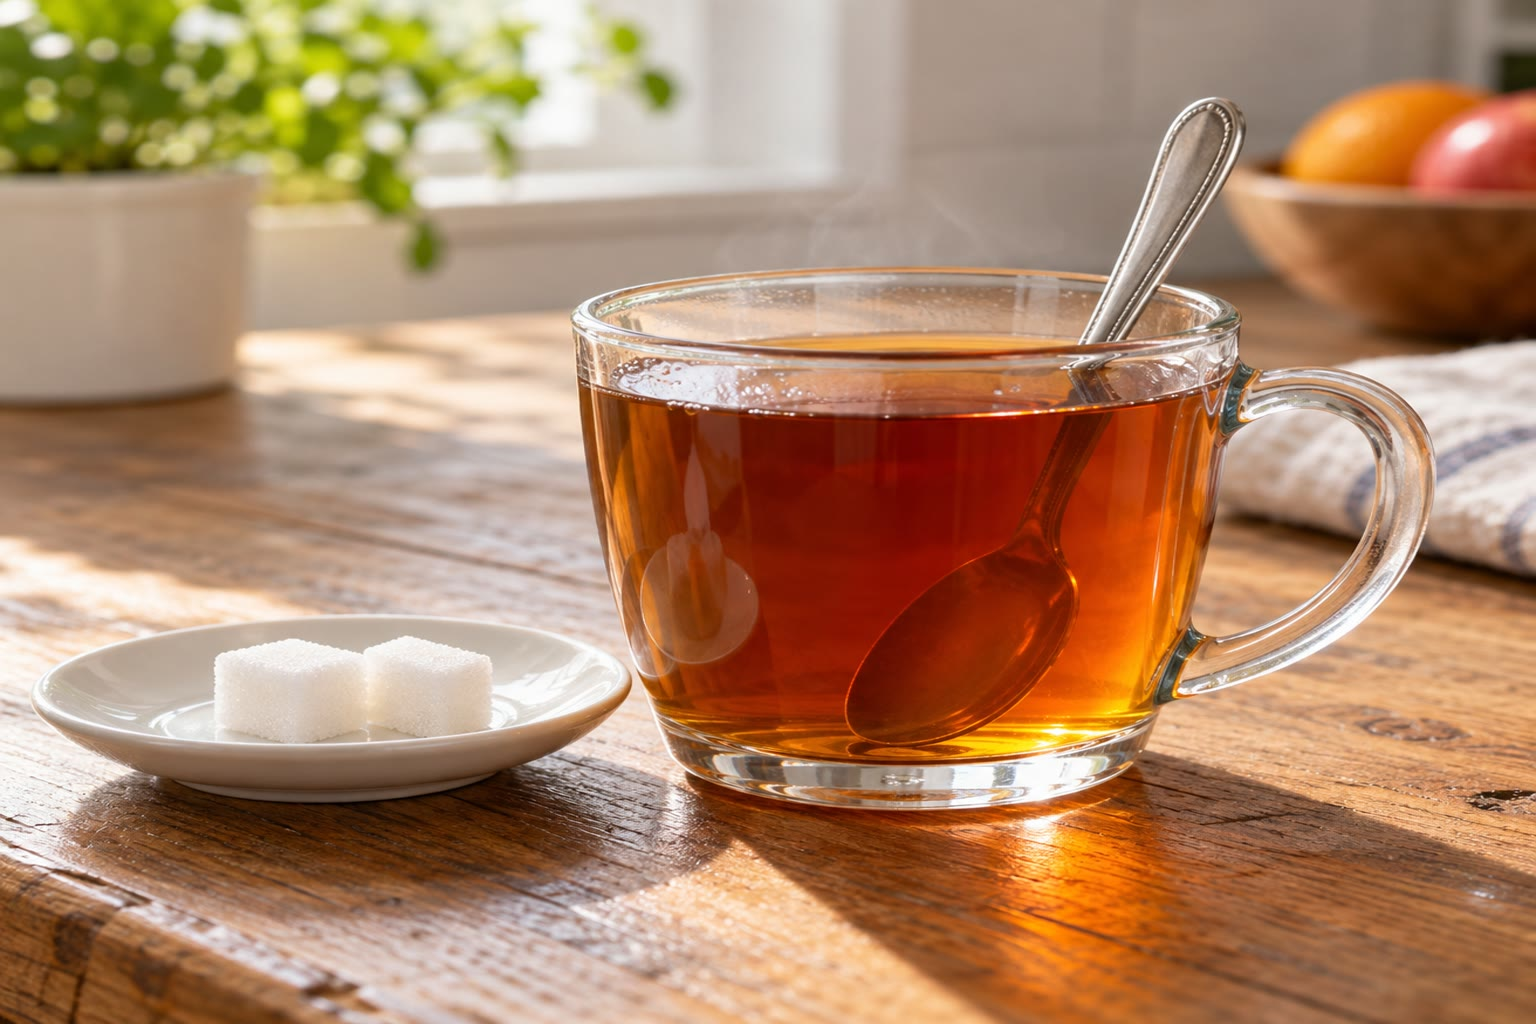
\includegraphics[width=0.55\linewidth]{images/book1/ai/g2-tea-sugar.jpg}

{\small Une tasse de thé et deux morceaux de sucre. Une fois remué, le
sucre disparaît à la vue, mais pas au goût.}
\end{omfigure}

\section{Mettre des choses ensemble}

\begin{definition}[Mélanger]\label{def:g2:mixing-and-dissolving:mix}
On \emph{mélange}\index{melanger@mélanger} des choses quand on les met ensemble,
souvent en les remuant. Ce que l'on obtient est un mélange de ces
choses.
\end{definition}

\begin{example}[Un bol de muesli]\label{ex:g2:mixing-and-dissolving:muesli}
On verse dans un même bol des flocons d'avoine, des raisins secs, des
noix et des graines~: c'est un \omterm{def:g2:mixing-and-dissolving:mix}{mélange}. En regardant de près, on voit
encore chaque ingrédient, et on peut le reprendre avec les doigts --- un
raisin reste un raisin, une noix reste une noix.
\end{example}

\begin{example}[Du sirop dans l'eau]\label{ex:g2:mixing-and-dissolving:syrup}
On peut aussi \omterm{def:g2:mixing-and-dissolving:mix}{mélanger} deux liquides. Du sirop rouge versé dans un verre
d'eau descend en volutes colorées~; après un coup de cuillère, tout le
verre est rose de façon égale. À l'œil, on ne peut plus distinguer le
sirop de l'eau.
\end{example}

\begin{omfigure}
\begin{minipage}[t]{0.48\linewidth}\centering
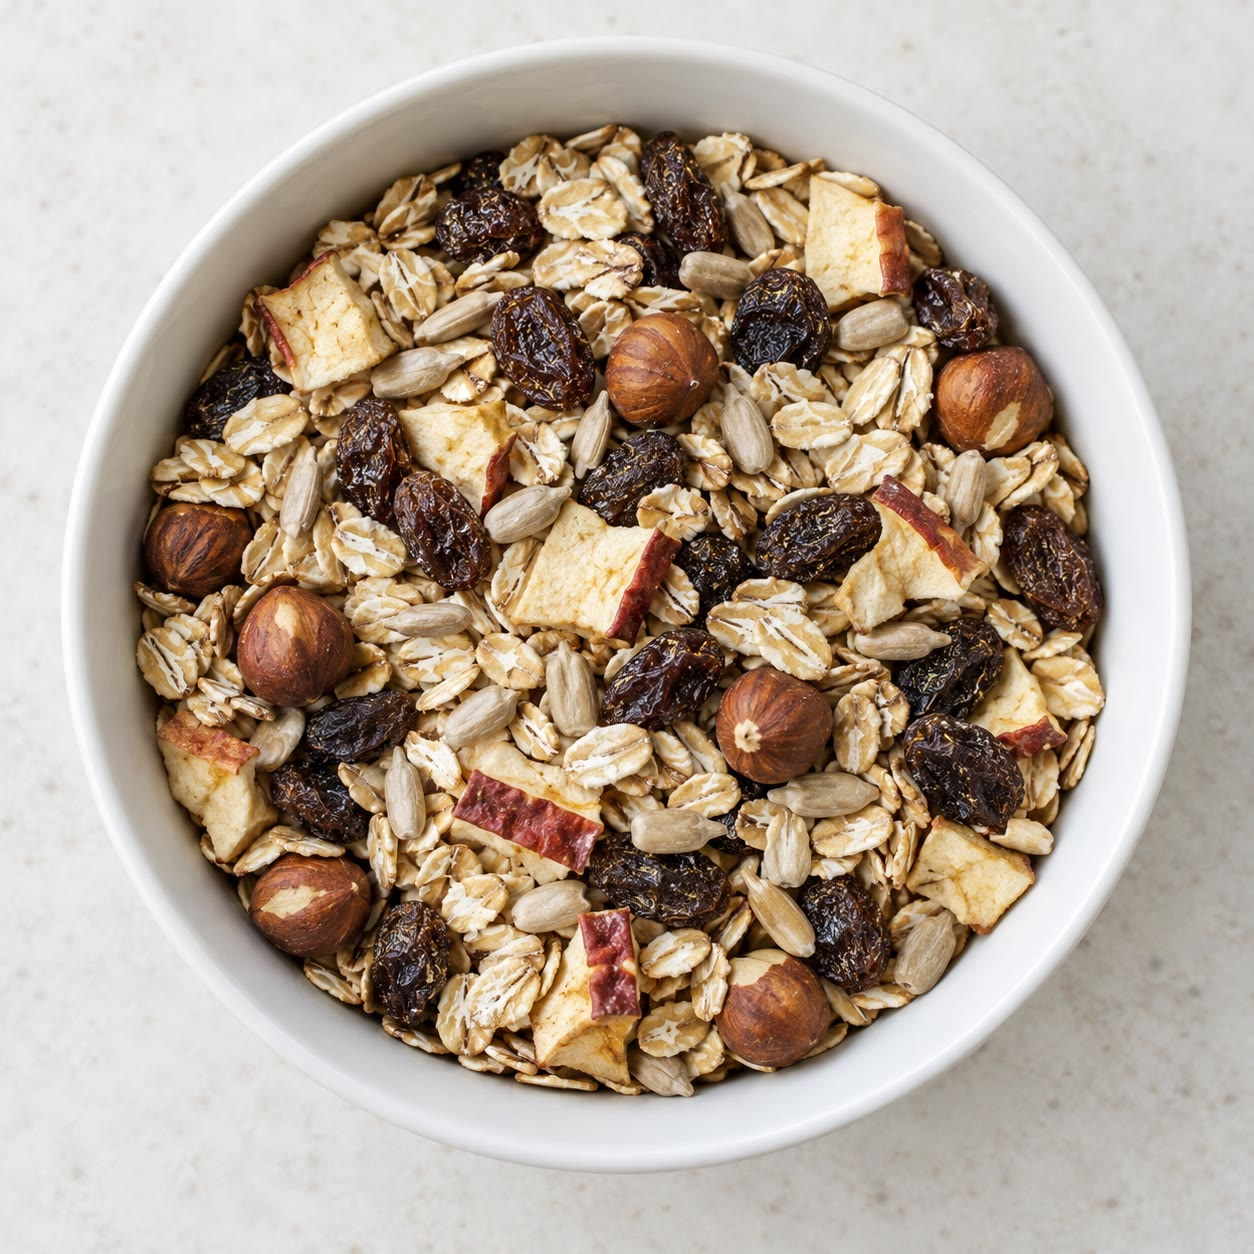
\includegraphics[width=\linewidth,height=4.6cm,keepaspectratio]{images/book1/ai/g2-muesli.jpg}

{\small Le muesli~: un \omterm{def:g2:mixing-and-dissolving:mix}{mélange} dont on voit encore chaque partie.}
\end{minipage}\hfill
\begin{minipage}[t]{0.48\linewidth}\centering
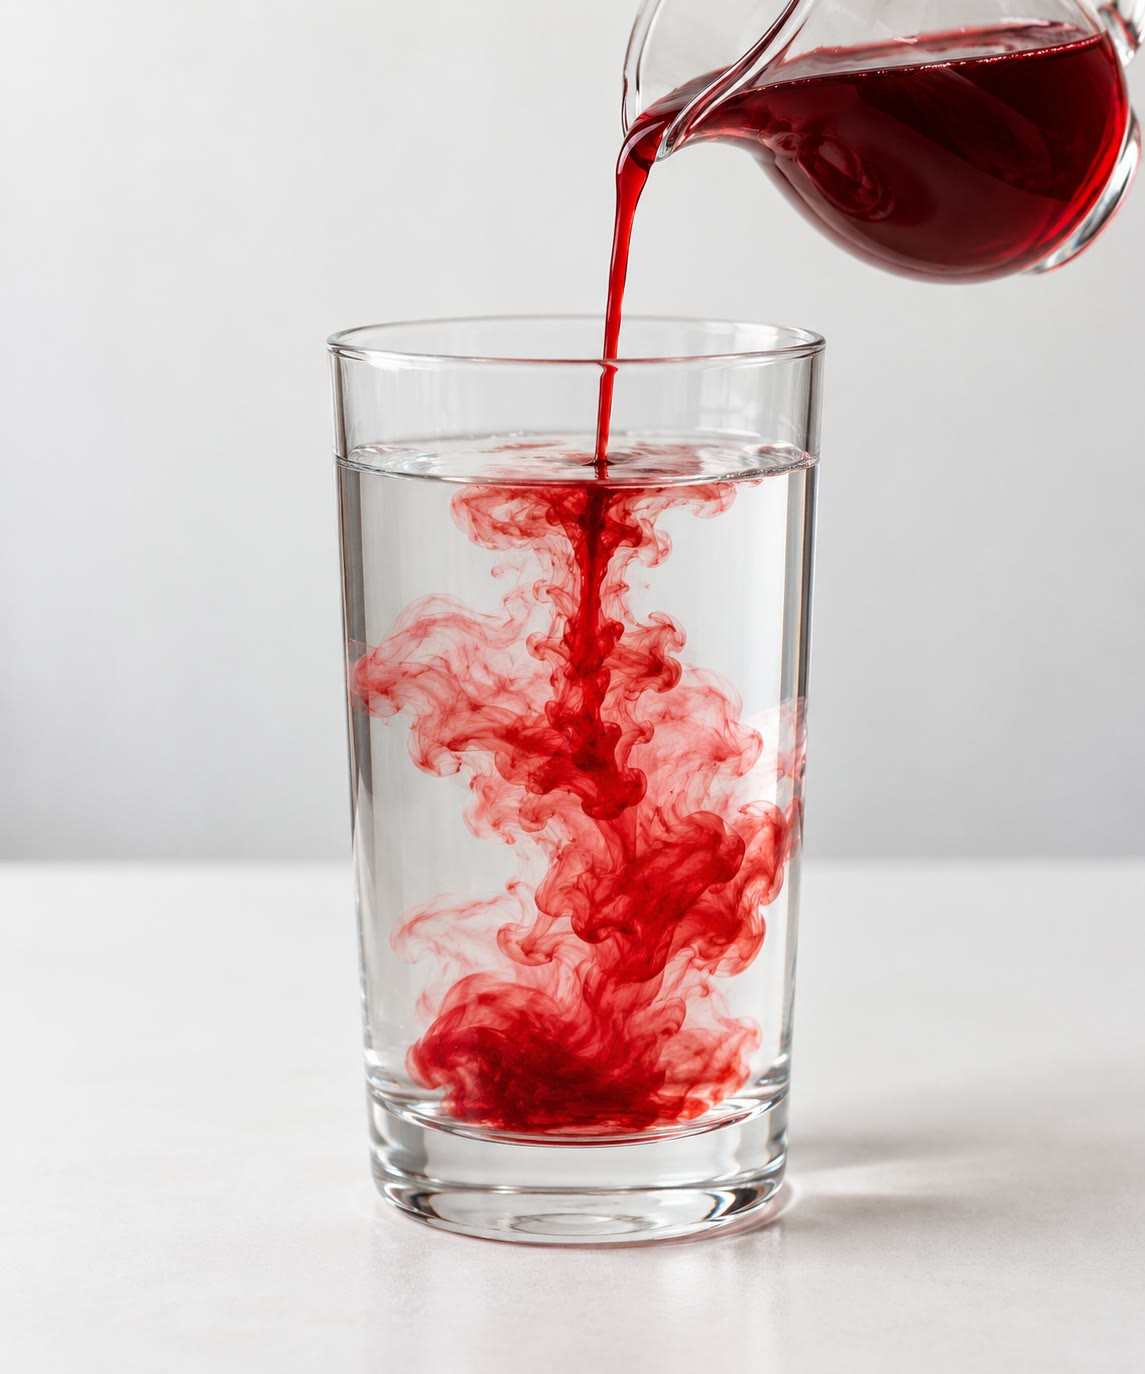
\includegraphics[width=\linewidth,height=4.6cm,keepaspectratio]{images/book1/ai/g2-syrup-in-water.jpg}

{\small Du sirop versé dans l'eau~: deux liquides qui se mélangent.}
\end{minipage}
\end{omfigure}

\begin{remark}[Mélanger ne détruit rien]\label{rem:g2:mixing-and-dissolving:nothing-lost}
Quand on \omterm{def:g2:mixing-and-dissolving:mix}{mélange} des choses, rien ne se perd et rien de nouveau n'est
fabriqué. Les flocons, les raisins et les noix sont toujours dans le bol.
Un chapitre suivant montre comment séparer à nouveau un \omterm{def:g2:mixing-and-dissolving:mix}{mélange}.
\end{remark}

\section{Ce qui se dissout}

\begin{definition}[Dissoudre, solution]\label{def:g2:mixing-and-dissolving:dissolve}
Un solide \emph{se dissout}\index{se dissoudre} dans l'eau quand, mis
dans l'eau et remué, il disparaît à la vue et laisse le liquide
\emph{limpide}, c'est-à-dire transparent. Le sucre et le sel se
dissolvent dans l'eau. Le liquide limpide obtenu s'appelle une
\emph{solution}\index{solution}~: l'eau sucrée est une solution de
sucre, l'eau salée une solution de sel.
\end{definition}

\begin{example}[Un morceau de sucre dans un verre d'eau]\label{ex:g2:mixing-and-dissolving:cube}
On pose un morceau de sucre au fond d'un verre d'eau immobile. Ses coins
s'arrondissent, il rapetisse, et des traînées ondulées montent de lui à
travers l'eau. Si l'on remue, il a disparu en moins d'une minute. Si
l'on ne remue pas, il disparaît quand même, mais beaucoup plus
lentement.
\end{example}

\begin{remark}[Limpide ne veut pas dire incolore]\label{rem:g2:mixing-and-dissolving:clear}
Le thé est brun et l'eau au sirop est rose, mais on voit à travers les
deux~: ils sont limpides. Une \omterm{def:g2:mixing-and-dissolving:dissolve}{solution} peut avoir une couleur. Ce
qu'une \omterm{def:g2:mixing-and-dissolving:dissolve}{solution} n'a jamais, ce sont des morceaux qui flottent dedans ou
une couche au fond.
\end{remark}

\begin{method}[Est-ce que ça se dissout~?]\label{met:g2:mixing-and-dissolving:test}
Pour savoir si un solide \omterm{def:g2:mixing-and-dissolving:dissolve}{se dissout} dans l'eau~:
\begin{enumerate}
  \item mets un peu du solide dans un verre d'eau~;
  \item remue, puis attends quelques minutes~;
  \item regarde à travers le verre~:
    \begin{itemize}
      \item limpide, et rien au fond~: le solide s'est dissous~;
      \item trouble, ou une couche au fond~: le solide ne s'est pas
            dissous.
    \end{itemize}
\end{enumerate}
\end{method}

\section{Ce qui ne se dissout pas}

\begin{proposition}[Le sable et la craie ne se dissolvent pas]\label{prop:g2:mixing-and-dissolving:not}
Beaucoup de solides ne se dissolvent pas dans l'eau~: le sable, la
craie, la terre, les cailloux, la farine. Remués dans l'eau, ils la
rendent trouble~; laissés au repos, ils descendent et se déposent au
fond, et l'eau au-dessus redevient plus claire. On a beau remuer
longtemps, ils ne disparaissent jamais.
\end{proposition}

\begin{example}[Un bocal d'eau boueuse]\label{ex:g2:mixing-and-dissolving:mud}
De la terre du jardin secouée dans un bocal d'eau la rend brune et
trouble. Au bout d'une heure, la terre et les petits cailloux forment
une couche sombre au fond, quelques feuilles mortes flottent en
surface, et l'eau entre les deux n'est plus que légèrement trouble. La
terre ne s'est pas dissoute.
\end{example}

\begin{omfigure}
\begin{minipage}[t]{0.48\linewidth}\centering
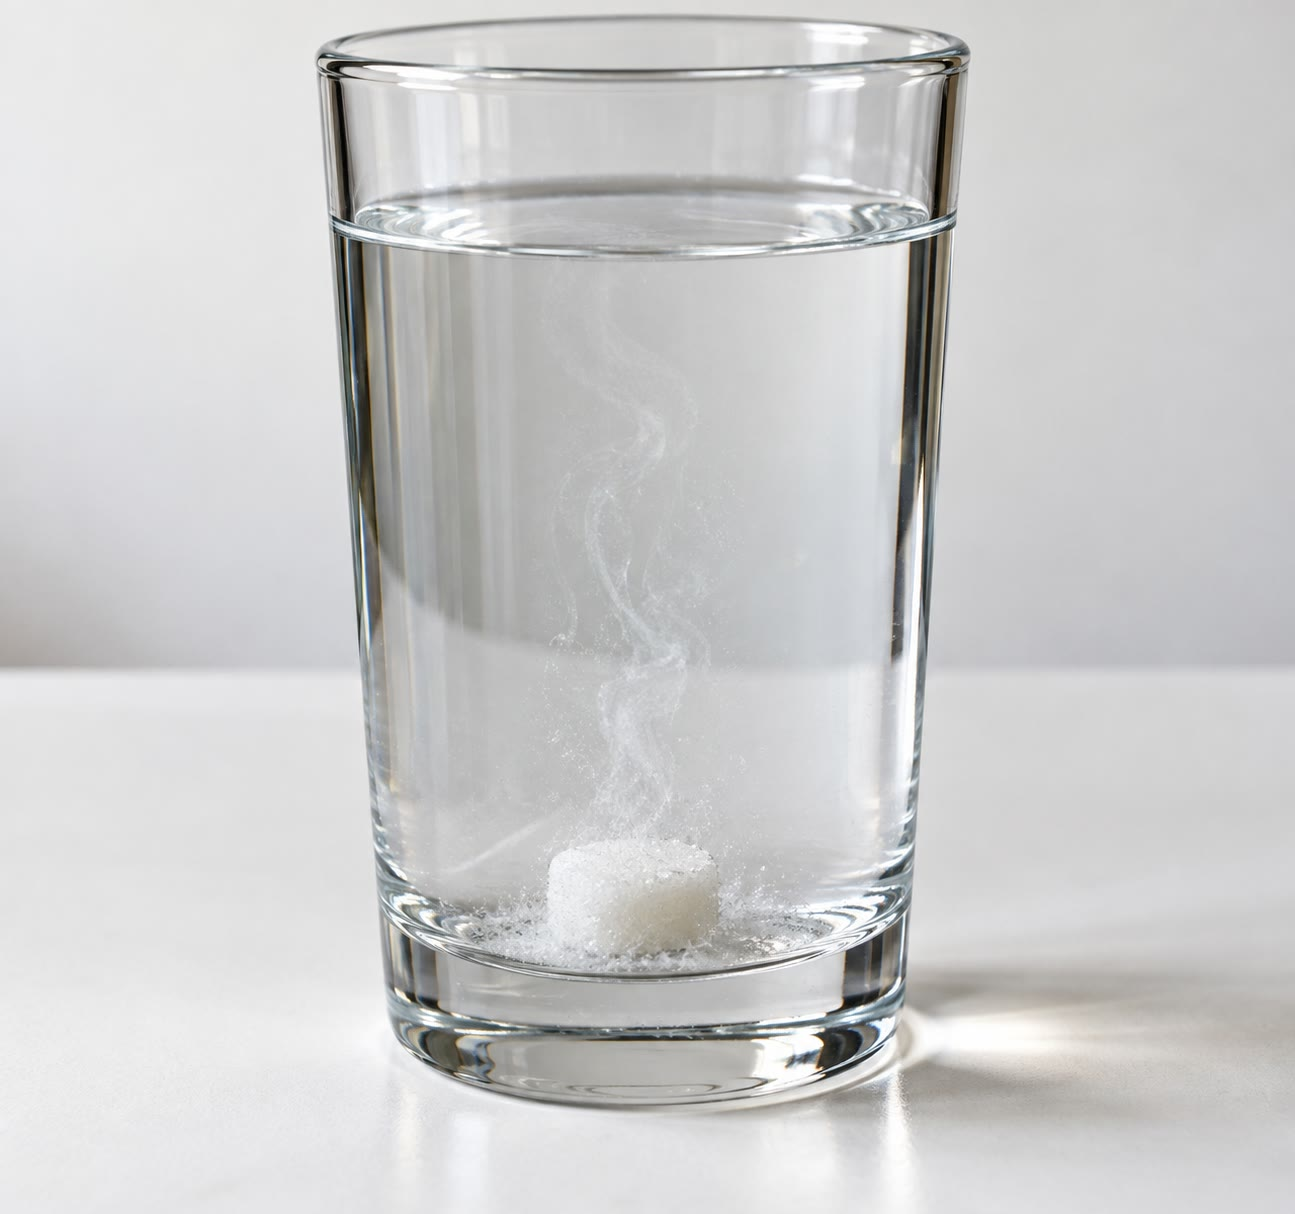
\includegraphics[width=\linewidth,height=4.6cm,keepaspectratio]{images/book1/ai/g2-sugar-cube-dissolving.jpg}

{\small Le sucre \omterm{def:g2:mixing-and-dissolving:dissolve}{se dissout}~: des traînées montent du morceau.}
\end{minipage}\hfill
\begin{minipage}[t]{0.48\linewidth}\centering
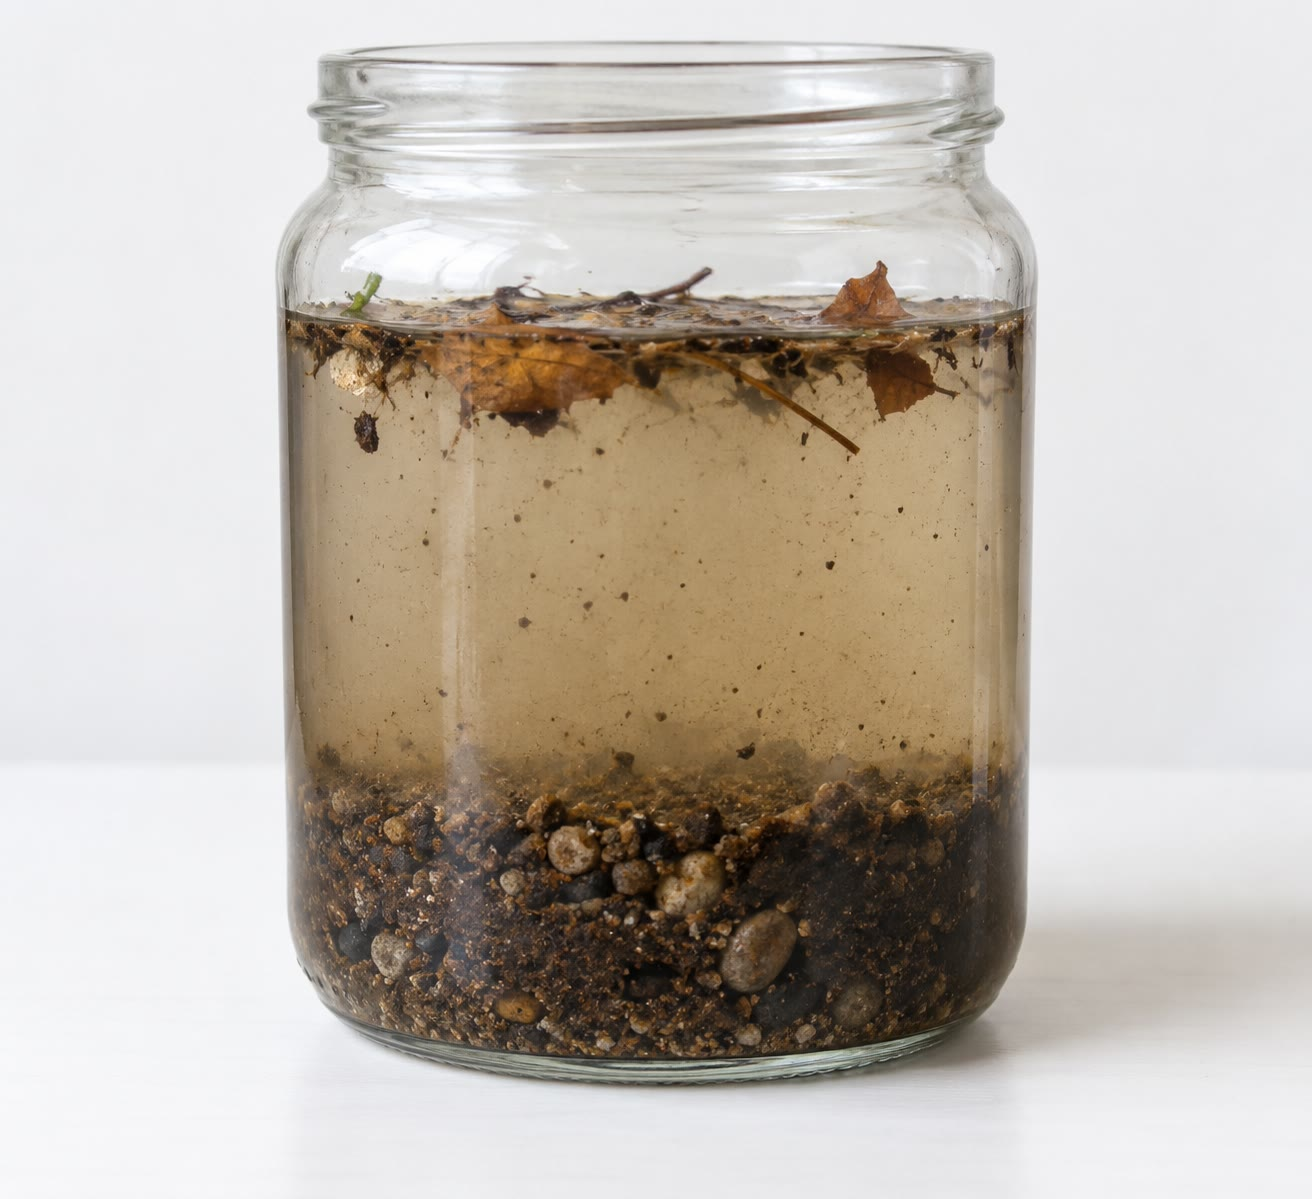
\includegraphics[width=\linewidth,height=4.6cm,keepaspectratio]{images/book1/ai/g2-muddy-jar.jpg}

{\small La terre ne \omterm{def:g2:mixing-and-dissolving:dissolve}{se dissout} pas~: elle se dépose au fond.}
\end{minipage}
\end{omfigure}

\begin{omfigure}
\begin{tikzpicture}[font=\small, scale=1.35]
  \pic[transform shape] at (0,0) {beaker={0.7}{omWater!70}};
  \fill[brown!55] (4.2,0) rectangle (5.8,0.22);
  \pic[transform shape] at (5,0) {beaker={0.7}{brown!12}};
  \fill[brown!55] (4.2,0) rectangle (5.8,0.22);
  \draw[omGlass, line width=0.7pt] (4.2,0.22) -- (4.2,0) -- (5.8,0) -- (5.8,0.22);
  \foreach \x/\y in {4.4/0.32,4.75/0.45,5.1/0.3,5.5/0.5,4.6/0.7,5.3/0.8,4.9/1.0}
    \fill[brown!60] (\x,\y) circle (0.025);
  \node[align=center, anchor=north] at (0,-0.15)
    {\textbf{sucre} dans l'eau, remué~:\\ limpide, rien au fond};
  \node[align=center, anchor=north] at (5,-0.15)
    {\textbf{sable} dans l'eau, remué~:\\ trouble, une couche au fond};
  \draw[<-, omProp, thick] (6.0,0.11) -- (7.0,0.11)
    node[right, text=black] {le sable};
\end{tikzpicture}

{\small Le test de la \cref{met:g2:mixing-and-dissolving:test}~: le sucre
\omterm{def:g2:mixing-and-dissolving:dissolve}{se dissout}, le sable non.}
\end{omfigure}

\section{Ce qui est dissous est toujours là}

\begin{proposition}[Un solide dissous est toujours dans l'eau]\label{prop:g2:mixing-and-dissolving:still-there}
Quand un solide \omterm{def:g2:mixing-and-dissolving:dissolve}{se dissout}, il ne disparaît pas~: il est réparti dans
toute l'eau, en morceaux bien trop petits pour être vus. Deux indices
montrent qu'il est toujours là~:
\begin{itemize}
  \item le thé sucré a un goût sucré, et l'eau de mer un goût salé~;
  \item quand l'eau s'évapore jusqu'à sécher, le solide reste.
\end{itemize}
\end{proposition}

\begin{remark}[On ne goûte rien au laboratoire]\label{rem:g2:mixing-and-dissolving:no-tasting}
On sait que le thé est sucré parce que le thé est un aliment. Au
laboratoire, personne ne goûte jamais rien, pas même un liquide qui
ressemble à de l'eau~: le second indice, laisser l'eau sécher, est
celui qu'utilisent les chimistes.
\end{remark}

\begin{example}[Le sel de la mer]\label{ex:g2:mixing-and-dissolving:salt-pans}
Sur certaines côtes ensoleillées, on fait entrer l'eau de mer dans de
grands bassins peu profonds. Jour après jour, le soleil fait sécher
l'eau. Ce qui reste au fond est du sel blanc, que l'on ramasse en tas~:
c'est le sel qui était dissous dans la mer. Le sel de la table vient
souvent de ces bassins, qu'on appelle des marais salants.
\end{example}

\begin{omfigure}
\begin{tikzpicture}[font=\small, scale=1.25]
  % day 1: a saucer of salty water
  \fill[omWater!80] (0,0.18) ellipse (1.25 and 0.22);
  \draw[omGlass, line width=0.7pt] (-1.5,0.3) .. controls (-1.2,-0.15) and (1.2,-0.15) .. (1.5,0.3);
  \draw[omGlass, line width=0.5pt] (0,0.3) ellipse (1.5 and 0.28);
  \node[align=center, anchor=north] at (0,-0.35) {une soucoupe\\ d'eau salée};
  % the sun
  \fill[ocYellow] (3.4,1.45) circle (0.28);
  \foreach \a in {0,45,...,315}
    \draw[ocYellow!90!orange, thick] ($(3.4,1.45)+(\a:0.36)$) -- ($(3.4,1.45)+(\a:0.52)$);
  \draw[->, thick, omProp] (2.0,0.3) -- (4.8,0.3)
    node[midway, below, text=black, align=center] {quelques jours\\ de soleil plus tard};
  % later: a white crust
  \begin{scope}[xshift=6.3cm]
    \draw[omGlass, line width=0.7pt] (-1.5,0.3) .. controls (-1.2,-0.15) and (1.2,-0.15) .. (1.5,0.3);
    \draw[omGlass, line width=0.5pt] (0,0.3) ellipse (1.5 and 0.28);
    \foreach \x/\y in {-0.9/0.12,-0.6/0.2,-0.3/0.08,0/0.18,0.3/0.1,0.6/0.2,0.9/0.12,
                       -0.45/0.28,0.15/0.27,0.75/0.3,-0.75/0.31}
      \fill[white, draw=black!45, line width=0.2pt] (\x,\y) rectangle ++(0.11,0.07);
    \node[align=center, anchor=north] at (0,-0.35) {plus d'eau~:\\ du sel blanc};
  \end{scope}
\end{tikzpicture}

{\small L'eau sèche~; le sel qui y était dissous reste.}
\end{omfigure}

\begin{omfigure}
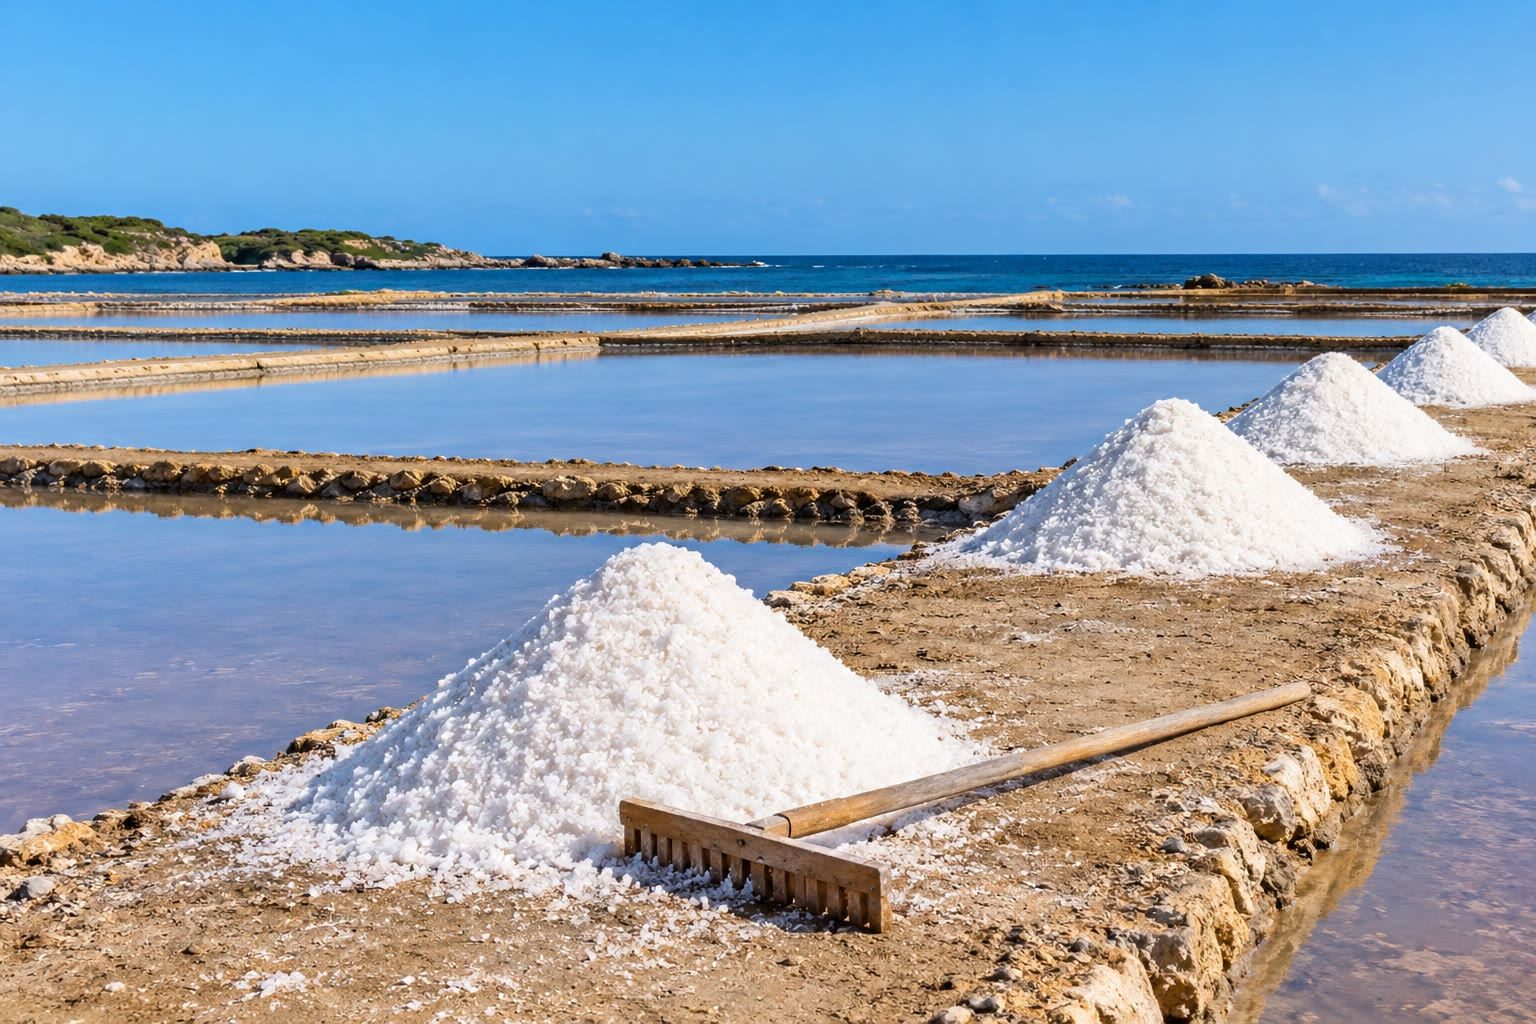
\includegraphics[width=0.62\linewidth]{images/book1/ai/g2-salt-pans.jpg}

{\small Des marais salants au bord de la mer~: le soleil fait sécher
l'eau, le sel reste en tas blancs.}
\end{omfigure}

\begin{remark}[Se dissoudre, ce n'est pas fondre]\label{rem:g2:mixing-and-dissolving:not-melting}
On dit souvent que le sucre «~fond~» dans le thé. Ce n'est pas vrai~:
fondre, c'est ce que fait un glaçon au soleil, quand il devient liquide
tout seul, sans avoir besoin d'eau. Le sucre dans le thé a besoin de
l'eau, et le sucre est toujours dedans, réparti. Le mot juste est
\emph{\omterm{def:g2:mixing-and-dissolving:dissolve}{se dissout}}.
\end{remark}

\section{Exercices}

\begin{exercise}[$\star$]\label{exo:g2:mixing-and-dissolving:1}
Parmi ces solides, lesquels se dissolvent dans l'eau, et lesquels ne se
dissolvent pas~? Le sucre, le sable, le sel, la craie, les cailloux.
\end{exercise}

\begin{exercise}[$\star$]\label{exo:g2:mixing-and-dissolving:2}
Qu'est-ce qu'une \omterm{def:g2:mixing-and-dissolving:dissolve}{solution}~? Donne deux exemples tirés de ce chapitre.
\end{exercise}

\begin{exercise}[$\star$]\label{exo:g2:mixing-and-dissolving:3}
Un bol de muesli est-il un \omterm{def:g2:mixing-and-dissolving:mix}{mélange}~? Peux-tu encore voir chacune de ses
parties~?
\end{exercise}

\begin{exercise}[$\star$]\label{exo:g2:mixing-and-dissolving:4}
On remue une poudre blanche dans un verre d'eau. Au bout de quelques
minutes, l'eau est trouble et une couche blanche s'est formée au fond.
La poudre s'est-elle dissoute~? Explique avec la
\cref{met:g2:mixing-and-dissolving:test}.
\end{exercise}

\begin{exercise}[$\star$]\label{exo:g2:mixing-and-dissolving:5}
Un verre d'eau au sirop est rose. Est-il limpide~? Est-il incolore~?
Est-ce une \omterm{def:g2:mixing-and-dissolving:dissolve}{solution}~?
\end{exercise}

\begin{exercise}[$\star$]\label{exo:g2:mixing-and-dissolving:6}
Après avoir remué, on ne voit plus de sucre dans une tasse de thé.
Donne l'indice qui montre que le sucre est toujours là.
\end{exercise}

\begin{exercise}[$\star$]\label{exo:g2:mixing-and-dissolving:7}
Dans les marais salants, qu'est-ce que le soleil enlève, et qu'est-ce
qui reste~?
\end{exercise}

\begin{exercise}[$\star$]\label{exo:g2:mixing-and-dissolving:8}
Tom dit~: «~Le sucre a fondu dans mon thé.~» Quel mot devrait-il
employer à la place, et pourquoi~?
\end{exercise}

\begin{exercise}[$\star\star$]\label{exo:g2:mixing-and-dissolving:9}
Regarde la figure des deux béchers. Sans lire les mots écrits dessous,
comment peux-tu savoir quel bécher contient le sable~?
\end{exercise}

\begin{exercise}[$\star\star$]\label{exo:g2:mixing-and-dissolving:10}
Une goutte d'eau du robinet sèche sur une assiette noire et laisse un
petit cercle blanc. Qu'est-ce que cela nous apprend sur l'eau du
robinet~?
\end{exercise}

\begin{exercise}[$\star\star$]\label{exo:g2:mixing-and-dissolving:11}
Au laboratoire, une professeure a deux verres d'un liquide limpide et
incolore~: l'un contient de l'eau pure, l'autre de l'eau salée.
Personne n'a le droit d'y goûter. Comment peut-elle savoir lequel est
lequel~?
\end{exercise}
